% ---- ETD Document Class and Useful Packages ---- %
\documentclass{ucetd}
\usepackage{subfigure,epsfig,amsfonts}
\usepackage{natbib}
\usepackage{amsmath}
\usepackage{amssymb}
\usepackage{amsthm}
\usepackage[toc,page]{appendix}
\usepackage[labelfont=bf]{caption}
\usepackage{rotating}
\usepackage[dvipsnames]{xcolor}
\usepackage{url}
\usepackage{bm}

%% Use these commands to set biographic information for the title page:
\title{The statistical mechanics of transcriptional control}
\author{Clayton W. Seitz}
\department{Department of Physics}
\division{Physical Sciences}
\degree{Doctor of Philosophy}
\date{Spring 20XX}

%% Use these commands to set a dedication and epigraph text

\epigraph{Epigraph}



\begin{document}
%% Basic setup commands
% If you don't want a title page comment out the next line and uncomment the line after it:
\maketitle
%\omittitle

% These lines can be commented out to disable the copyright/dedication/epigraph pages
\makecopyright
%\makededication


%% Make the various tables of contents
\tableofcontents
%\listoffigures
%\listoftables

%\acknowledgments
% Enter Acknowledgements here

\abstract

Eukaryotic transcription is episodic, consisting of a series of transcriptional bursts, Bursty transcriptional dynamics are well-exemplified by the transient expression of pro-inflammatory guanylate binding proteins (GBPs) - a group interferon-inducible GTPases that restrict the replication of intracellular pathogens [XXX]. Classical models of gene regulation explain transcriptional bursts by invoking stochastic binding and unbinding of transcription factors, RNA polymerase and mediator proteins at enhancer or promoter sequences. However, more recent studies have pointed towards a more cooperative picture of transcriptional control where phase-separated aggregates of DNA, RNA, and proteins form higher-order structures to control gene expression. For example, both chromatin immunoprecipitation and super resolution imaging have captured the phase separation of super-enhancer-binding proteins MED1 and BRD4 in transcriptional condensates at the \textit{Essrb} genomic locus [XXX]. Furthermore, fluorescence microscopy techniques have colocalized MED1 and BRD4 with the GBP gene cluster alongside a reduction in the degree of disorder of 3D chromatin structure in murine macrophages after infection with \textit{Mycobacterium tuberculosis}. Taken together, these results suggest that phase separation may play a role in the reorganization of chromatin structure during trancriptional control of innate immune response genes [XXX]. Here, we hypothesize that phase separation reduces the entropy of chromatin structure in order to induce bursty gene expression. Using single molecule localization microscopy (SMLM) to obtain super-resolution images of the H2B protein, we intend to demonstrate simultaneous (i) loss of disorder in chromatin structure (ii) formation of transcriptional condensates containing MED1 and BRD4 and (iii) non-Poissonian gene expression. The following sections discuss recent the biological evidence in more detail and summarize the single molecule microscopy techniques and biophysical models we employ to study the interactions between transcriptional condensates and the chromatin scaffold.

\clearpage

\mainmatter

\chapter{Single molecule localization microscopy}

\section{Point spread functions in single molecule localization microscopy}

Gaussian approximation. Lateral and axial point spread functions, Potentially double helix point spread functions for 3D storm

Most detectors used for imaging have many elements (pixels) so that we can record an image projected onto the detector by a system of lenses. In fluorescence imaging, this is usually a relay consisting of an objective lens and a tube lens to focus the image onto the camera. Due to diffraction, any point emitter, such as a single fluorescent molecule, will be registered as a diffraction limited spot. The profile of that spot is often described as a Gaussian point spread function (Richardson and Wolf)

\begin{equation}
\mathrm{G}(x,y) = \frac{1}{2\pi\sigma^{2}}e^{-\frac{(x-x_{0})^{2}+(y-y_{0})^{2}}{2\sigma^{2}}} + B_0
\end{equation}

which has units of $[W/m^{2}]$.

\begin{figure}[t!]
\centering
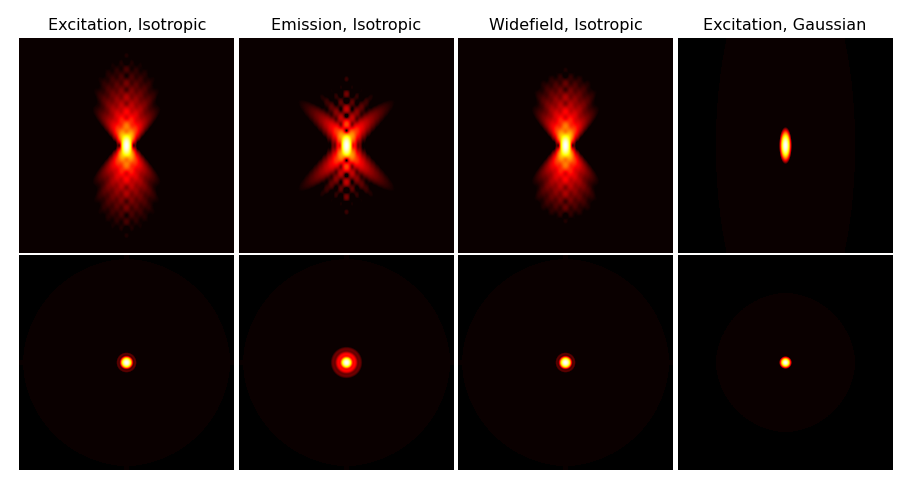
\includegraphics[width=150mm]{psf-1}
\end{figure}

\begin{figure}[t!]
\centering
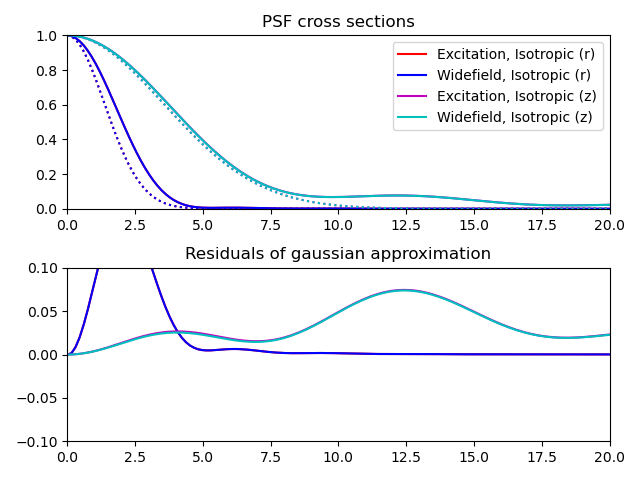
\includegraphics[width=150mm]{psf-2}
\end{figure}

\begin{figure}[t!]
\centering
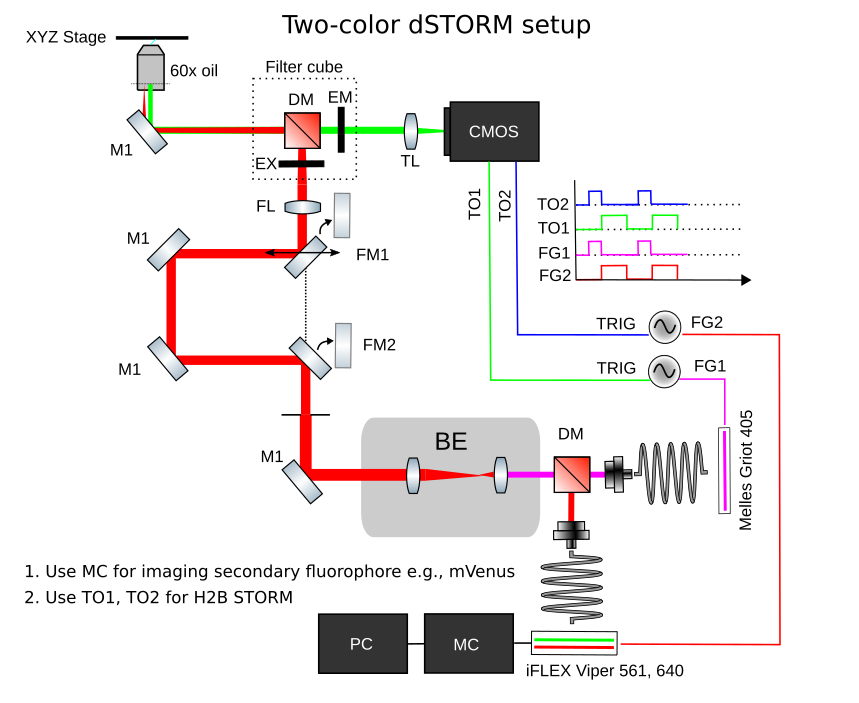
\includegraphics[width=150mm]{dSTORM}
\end{figure}

\subsection{The physics of semiconductor cameras}

Modern cameras used in light microscopy, such as scientific complementary metal oxide semiconductor (sCMOS) cameras, are ultimately powered by the photoelectric effect. This occurs when electrons within the material absorb energy from the photons and have enough energy to escape their bonds and become ejected from the material. The materials used in camera sensors are typically semiconductors such as silicon or gallium

In essence, an image captured by a camera can be loosely thought of as histogram of photon arrivals and a discretized form of the density $\mathrm{PSF}(x,y)$ over an integration time $\tau$. If $\mathrm{PSF}(x,y)$ can be approximated as constant in time, the value at a pixel approaches an integral of this density over the pixel:

\begin{equation}
\mu_{k} = \lambda_{k}\tau = \frac{\eta\tau}{\hbar\omega}\int G(x,y)dA
\end{equation}

The parameter $\eta$ is called the \emph{quantum efficiency}, and without loss of generality, we will assume $\eta = 1$. The variable $\lambda_{k}$ at a pixel $k$ defines the probability of observing a photon per unit time and the \emph{true signal} is Poisson: $S_{k} \sim P(\lambda_{k})$. In this model, notice that $S_{k}$ may represent multiple sources e.g., fluorescence from a single molecule plus a background source as shown in (1.1). Furthermore, we say that the detection process is \emph{shot-noise limited} when Poisson noise dominates. It would be convenient to obtain an analytical expression for $\lambda_{k}$ given the parameters of the point spread function $\theta = (x_0,y_0,\sigma)$. Since the 2D Gaussian is symmetric, it is separable, and we can write

\begin{align*}
\lambda_{k} &= \frac{1}{2\pi\sigma^{2}}\left(\int_{x_{k}}^{x_{k+1}}e^{-\frac{(x-x_{0})^{2}}{2\sigma^{2}}}dx\right)\left(\int_{y_{k}}^{y_{k+1}}e^{-\frac{(y-y_{0})^{2}}{2\sigma^{2}}}dy\right)
\end{align*}

\begin{figure}[t!]
\centering
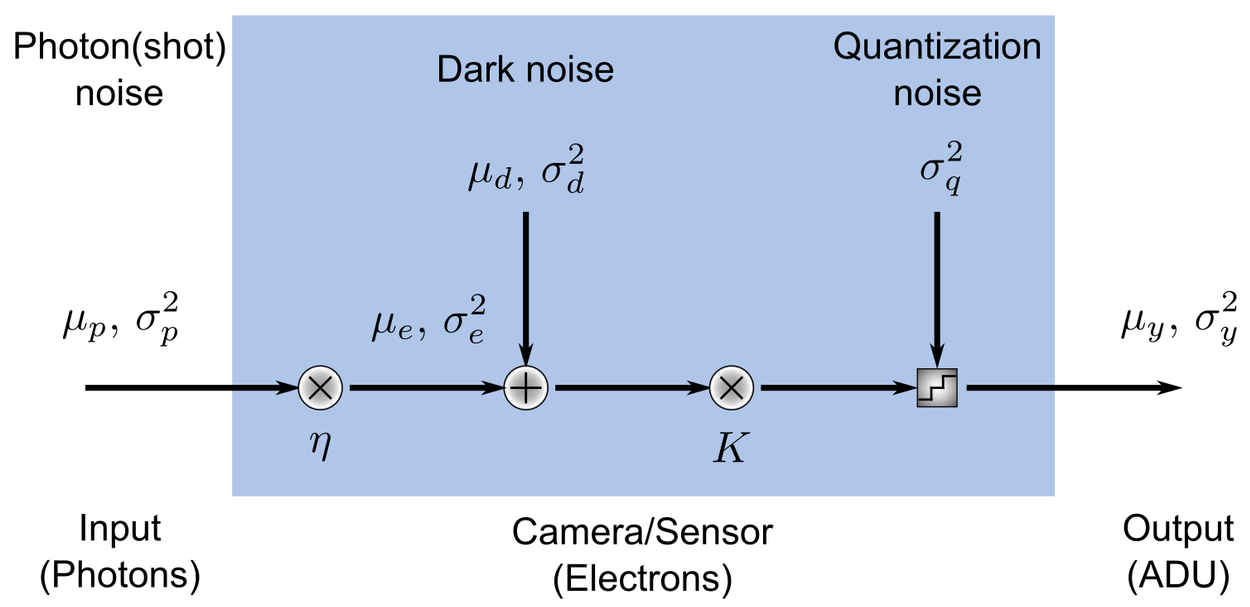
\includegraphics[width=150mm]{noise-model}
\end{figure}

We can then express the Gaussian integrals over a pixel by making use of the following property of the error function

\begin{equation*}
\frac{1}{\sqrt{2\pi}\sigma}\int_{a}^{b} e^{\frac{-(x-\mu)^{2}}{2\sigma^{2}}} = \frac{1}{2}\left(\mathrm{erf}\left(\frac{b-\mu}{\sqrt{2}\sigma}\right) -\mathrm{erf}\left(\frac{a-\mu}{\sqrt{2}\sigma}\right)\right)
\end{equation*}

Suppose the particle is known to be located at $(x_{0},y_{0})$ and some square pixel $k$ is centered on coordinates $(x,y)$ and has a width $a$. Then $\lambda_{k}$ at this pixel is

\begin{align*}
\lambda_{k} &= \frac{1}{4}\left(\mathrm{erf}\left(\frac{x+a/2-x_{0}}{\sqrt{2}\sigma}\right) -\mathrm{erf}\left(\frac{x-a/2-x_{0}}{\sqrt{2}\sigma}\right)\right)\\
&\cdot \left(\mathrm{erf}\left(\frac{y+a/2-y_{0}}{\sqrt{2}\sigma}\right) -\mathrm{erf}\left(\frac{y-y/2-y_{0}}{\sqrt{2}\sigma}\right)\right)
\end{align*}

However this noise model is incomplete, because detectors often suffer from dark noise, which may refer to readout noise or dark current, and contributes to a nonzero signal even in the absence of incident light. Dark current is due to statistical fluctuations in the photoelectron count due to thermal fluctuations. Readout noise is introduced by the amplifier circuit during the coversion of photoelectron charge to a voltage. Here, we use the Hamamatsu ORCA v3 CMOS camera, which is air cooled to -10C and has very low dark current - around 0.06 electrons/pixel/second - and can be safely ignored for low exposure times. Readout noise has been often neglected in localization algorithms because its presence in EMCCD cameras is small enough that it can be ignored within the tolerances of the localization precision. In the case of sCMOS cameras, however, the readout noise of each pixel is significantly higher and, in addition, every pixel has its own noise and gain characteristic with dramatic pixel-to-pixel variations.

Readout noise is not negligible, and is represented as a random variable $W_{k}$ which is \textit{a statistical fluctuation of the number of ADU during the amplification process}. It is important to note that we cannot measure the contribution by readout noise $W_{k}$ before amplification and therefore it must be expressed in units of $\mathrm{ADU}$. This is in contrast to the Poisson variable $S_{k}$, which \emph{can} be expressed in units of photoelectrons, because we are able to estimate the emission rate of the fluorophore analytically and we know the quantum efficiency $\eta$. The number of photoelectrons $S_{k}$ is  multiplied by a gain factor $g_{k}$ which has units of $[\mathrm{ADU}/e^{-}]$, which generally must be measured for each pixel. For $W_{k}$, the gain factor is implied. Here, we will always assume that readout noise is Gaussian with some pixel-specific offset $o_{k}$ and variance $\sigma_{k}^{2}$ i.e. $W_{k} \sim \mathcal{N}(o_{k},\sigma_{k}^{2})$. Ultimately we write out distributions of the variable we observe $H_{k}$ which has units of $\mathrm{ADU}$ and is a sum of shot noise and readout noise. A fundamental result in probability theory is that the distribution of $H_{k}$ is the convolution of the distributions of $S_{k}$ and $W_{k}$,

\begin{align*}
P(H_{k}|\theta) &= P(S_{k})\circledast P(W_{k})\\
&= A\sum_{q=0}^{\infty} \frac{1}{q!}e^{-\mu_{k}}\mu_{k}^{q}\frac{1}{\sqrt{2\pi}\sigma_{k}}e^{-\frac{(H_{k}-g_{k}q-o_{k})}{2\sigma_{k}^{2}}}
\end{align*}

In practice, this expression is difficult to work with, so we look for an analytical approximation. For sufficiently large $\mu_{k}$, the Poisson distribution is well-approximated by a normal distribution $P(\mu_{k}) \approx \mathcal{N}(\mu_{k},\mu_{k})$. Under the conditions that this approximation is valid, $P(H_{k})$ is easily calculated, because the sum of two Gaussian variables is another Gaussian variable:

\begin{equation}
P(H_{k}|\theta) \approx \frac{1}{\sqrt{2\pi(\lambda_{k}\tau+\sigma_{k}^{2})}}e^{-\frac{(H_{k}-\lambda_{k}\tau-o_{k})}{2(\lambda_{k}\tau+\sigma_{k}^{2})}}
\end{equation}

Assuming each pixel is an independent random variable, then the likelihood of the dataset (or equivalently the joint distribution on pixels) is simply a product $\mathcal{L}(H|\theta) = \prod_{k}P(H_{k}|\theta)$. Now suppose we are given a sample from $\mathcal{L}(H|\theta)$ with unknown $\theta$. A general task in Bayesian inference is to determine $\theta$ from the data under the model $\mathcal{M}$. We may then ask - does the likelihood $\mathcal{L}$ vary as we vary the parameters? If the likelihood is flat, all parameter sets are equally likely and the data does not appear to carry much information about the parameters. Moreover, if $\mathcal{L}$ has a number of bumps or inflection points, then we expect that maybe some parameter sets are more likely that others. The ``bumpiness" of the likelihood surface is called the Fisher information. The Fisher information matrix $\mathbf{I}(\theta)$ can be directly related to the curvature of the KL-Divergence over the parameter space

\begin{align*}
\nabla^2_{\theta'} D_{KL}[\mathcal{L}(H|\theta) \parallel \mathcal{L}(H|\theta')] 
&= - \nabla_{\theta'} \int \mathcal{L}(H|\theta) \nabla_{\theta'}  \log \mathcal{L}(H|\theta') \, dH \\ 
&= - \int \mathcal{L}(H|\theta) \nabla^2_{\theta'}  \log \mathcal{L}(H|\theta') \, dH \\
&= - \mathbb{E}_{\theta}[\nabla^2_{\theta'} \log \mathcal{L}(H|\theta')] \\
&= \mathbf{I}(\theta)
\end{align*}

Luckily, we can directly compute the Hessian matrix of the log-likelihood $\nabla^2_{\theta'} \log \mathcal{L}(H|\theta')$. Moreover, from the expression above, we can see that it is convenient to work with the negative log-likelihood $\ell(H|\theta)$.

\begin{align*}
\nabla^2_{\theta'} \log \mathcal{L}(H|\theta') =
\begin{pmatrix}\frac{\partial^{2}\ell}{\partial x_{0}^{2}} & \frac{\partial\ell}{\partial x_{0}}\frac{\partial\ell}{\partial y_{0}} \\
\frac{\partial\ell}{\partial y_{0}}\frac{\partial\ell}{\partial x_{0}} &\frac{\partial^{2}\ell}{\partial y_{0}^{2}} 
\end{pmatrix}
\end{align*}

We begin by expanding $\ell(H|\theta)$:

\begin{align*}
\ell(H|\theta) &= \sum_{k} \ell(H_{k}|\theta) \\
&= \sum_{k} \log\sqrt{2\pi(\lambda_{k}\tau+\sigma_{k}^{2})}+\frac{(H_{k}-\lambda_{k}\tau-o_{k})}{2(\lambda_{k}\tau+\sigma_{k}^{2})}
\end{align*}

The Hessian can be constructed by differentiating this sum. The first order derivative w.r.t an arbitrary parameter is

\begin{align*}
\frac{\partial\ell(H|\theta)}{\partial \theta} &=  \sum_{k} \frac{\partial\ell_{k}(H_{k}|\theta)}{\partial \theta}\\
&= \sum_{k}\frac{\partial\ell_{k}(H_{k}|\theta)}{\partial \theta}\frac{\partial\lambda_{k}}{\partial \theta}
\end{align*}

and it is straightforward to show that 

\begin{align*}
\frac{\partial\ell_{k}}{\partial \lambda_{k}} = -\frac{(h-\lambda_{k} -\mu )^2}{2 \left(\lambda_{k} +\rho ^2\right)^2}-\frac{h-\lambda_{k} -\mu }{\lambda_{k} +\rho ^2}+\frac{1}{2 \left(\lambda_{k} +\rho ^2\right)}
\end{align*}

For $\theta = x_{0}$, we have

\begin{align*}
\frac{\partial\ell}{\partial x_{0}} = \frac{\tau\lambda_{y}}{2}\sum_{k} \frac{\partial\ell_{k}}{\partial \lambda_{k}}\left(\frac{\sqrt{\frac{2}{\pi }} e^{-\frac{\left(-\frac{a}{2}+x_{k}-\text{x0}\right)^2}{2 \sigma ^2}}}{\sigma }-\frac{\sqrt{\frac{2}{\pi }} e^{-\frac{\left(\frac{a}{2}+x_{k}-\text{x0}\right)^2}{2 \sigma ^2}}}{\sigma }\right)
\end{align*}



\begin{align*}
\theta^{*}_{\mathrm{MAP}} &= \underset{\theta}{\mathrm{argmax}} \;P(\theta|\mathcal{X})\\
&= \underset{\theta}{\mathrm{argmax}} \; \mathcal{L}(\theta|\mathcal{X})\pi(\theta)
\end{align*}


where $\mathcal{L}$ denotes the likelihood function (posterior probability of the parameters) and $\pi(\theta)$ a prior on the parameters. Under the constraint that $\pi(\theta)$ is a uniform distribution, we are dealing with maximum likelihood estimation

\begin{align*}
\theta^{*}_{\mathrm{MLE}} &= \underset{\theta}{\mathrm{argmax}} \;\mathcal{L}(\theta|\mathcal{X})\\
&= \underset{\theta}{\mathrm{argmin}} \; -\ell(\theta|\mathcal{X})
\end{align*}

where $\ell$ is the log-likelihood. 

We can now return to the original optimization problem 

\begin{align*}
\theta^{*}_{\mathrm{MAP}} &= \underset{\theta}{\mathrm{argmax}} \;\ \pi(\theta)\mathcal{L}_{\theta}\\
&= \underset{\theta}{\mathrm{argmax}} \; \prod_{k}\mathcal{L}_{\theta,k}\\
&= \underset{\theta}{\mathrm{argmax}} \; \sum_{k}\log \mathcal{L}_{\theta,k}
\end{align*}


\chapter{Statistical mechanics of gene regulation}

\section{Introduction}

\section{Transcriptional bursts and chromatin architecture}

\section{Transcriptional condensates: a phase separation model for transcriptional control}

Heavily influenced by Young's group at MIT


\section{Brief introduction to polymer dynamics}

\section{Statistical mechanics of transcriptional condensates}

\section{The chemical master equation and finite state projection}

The central assumption underlying a Markov process, is the memoryless property

\begin{equation*}
P(X_{t}|X_{t-1}, X_{t-2}, ..., X_{t-N}) = P(X_{t}|X_{t-1})
\end{equation*}

A single Markov chain is the set of states $\bm{X} = \{X_{1},X_{2},...,X_{N}\}$. Such a set can be generated provided that $P(X_{t}|X_{t-1})$ is known. To capture $P(X_{t}|X_{t-1})$ for all possible pairs $X_{t}$ and $X_{t-1}$, we define a square transition matrix $T\in \mathcal{R}^{N\times N}$ where $N = |\Omega|$. As such, the elements of $T$ represent the probability of a transition from a state $\omega_{j}$ to $\omega_{i}$ in a unit time

\begin{equation*}
T_{ij} = \mathrm{Pr}\left(X_{t}=\omega_{i}, | \;X_{t-1}=\omega_{j}\right)
\end{equation*}

Under these definitions, the row $T_{i}$ represents the present time, and is a conditional  probability distribution $P(\omega | X_{t-1} = \omega_{j})$ which requires that

\begin{equation*}
\sum_{j}T_{ij} = \sum_{j} P(X_{t} = \omega_{j} | X_{t-1} = \omega_{i}) = 1
\end{equation*}

The matrix $T$ is not necessarily symmetric $T_{ij} \neq T_{ji}$. One should note that the columns $T_{j}$ \emph{do not} define a probability distribution $P(X_{t} = \omega_{i} | X_{t-1} = \omega_{j})$ and therefore do not necessarily sum to unity. The probability $P(X_{t} = \omega_{i} | X_{t-1} = \omega_{j})$ has no meaning in this context, since we have defined the rows to represent a probability of the future given the present. We simply sample $X_{t} \sim P(X_{t} = \omega_{j} | X_{t-1} = \omega_{i})$, assign $i=j$, and repeat. It directly follows from the fundamental rules of probability, the first order dynamics for a \textbf{particular} state $\omega_{i}$: $P(\omega_{i},t)$ is given by

\begin{equation}
P(\omega_{i},t+dt) = P(\omega_{i},t) + \mathcal{J}_{i}dt
\end{equation}

The net probability current $\mathcal{J}_{i}$ must be 

\begin{equation*}
\mathcal{J}_{i} = \sum_{i}T_{ij}P(\omega_{j},t) - \sum_{j}T_{ij}P(\omega_{i},t)\\
\end{equation*}

The first is a sum on a column and the second a sum on a row. This can be simplified further by noticing that the normalization condition implies

\begin{align*}
T_{ij} &= 1 - \sum_{j}T_{ij}(1-\delta_{ij})\\
&= 1 - \sum_{j}T_{ij} + \sum_{j}T_{ij}\delta_{ij}
\end{align*}


\begin{align*}
\mathcal{J}_{i} &= \sum_{i}T_{ij}P(\omega_{j},t) - \sum_{j}T_{ij}P(\omega_{i},t)\\
&= \sum_{i}\left(1 - \sum_{j}T_{ij} + \sum_{j}T_{ij}\delta_{ij}\right)P(\omega_{j},t) - \sum_{j}T_{ij}P(\omega_{i},t)\\
&= |\Omega| - |\Omega| + \sum_{i}\sum_{j}T_{ij}P(\omega_{j},t)\delta_{ij} - \sum_{j}T_{ij}P(\omega_{i},t)\\
&= \sum_{j}T_{ji}P(\omega_{j},t) - T_{ij}P(\omega_{i},t)\\
\end{align*}

Notice that the Kronecker delta effectively just swaps the index. Taking the limit of (1.1), we arrive at the \textbf{master equation}


\begin{equation*}
\frac{\partial P(\omega_{i})}{\partial t} = \sum_{j}T_{ji}P(\omega_{j},t) - T_{ij}P(\omega_{i},t)
\end{equation*}

It is common to then define an operator $\bm{W}$ s.t. $W_{ij} = T_{ij}$ and $W_{ii} = -\sum_{j}T_{ij}$ 

\begin{align*}
\frac{dP(\omega_{i})}{dt} = \sum_{j}W_{ij}P(\omega_{j}) \rightarrow \frac{dP(\bm{\omega})}{dt} = \mathcal{J}(\bm{\omega}) = \mathbf{W}P(\bm{\omega})
\end{align*}

This operator form has a solution in terms of a matrix exponential

\begin{equation*}
P(\bm{\omega}, t) = \exp(\mathcal{J}(\bm{\omega}))
\end{equation*}

This matrix exponential is intractable for large $|\Omega|$. However, in the Finite State Projection algorithm, it is possible to truncate the state space $\Omega \rightarrow \tilde{\Omega}$ and obtain good estimates $\tilde{P}(\bm{\omega}, t)$ with some certificate of accuracy.

\subsection{Sequential tempered Markov Chain Monte Carlo}


\chapter{IFN-$\gamma$ induced transcriptional bursts}


\begin{appendices}
\chapter{Derivation of the Fokker Planck Equation}

\subsection{Kramers-Moyal Expansion}

Gixen many instantiations of a stochastic xariable $x$, we can construct a normalize histogram oxer all obserxations as a function of time $P(x,t)$. Howexer, in order to systematically explore the relationship between the parameterization of the process and $P(x,t)$ we require an expression for $\dot{P}(x,t)$. If we make a fundamental assumption that the exolution of $P(x,t)$ follows a Markox process i.e. its exolution has the memoryless property, then we can write

\begin{equation}
P(x', t) = \int T(x', t | x, t-\tau)P(x, t-\tau)dx
\end{equation} 

which is known at the Chapman-Kolmogorox equation. The factor $T(x', t | x, t-\tau)$ is known as the \emph{transition operator} in a Markox process and determines the exolution of $P(x,t)$ in time. We proceed by writing $T(x', t | x, t-\tau)$ in a form referred to as the Kramers-Moyal expansion

\begin{align*}
T(x', t | x, t-\tau) &= \int \delta(u-x')T(u, t | x, t-\tau)du\\
&= \int \delta(x+u-x'-x)T(u, t | x, t-\tau)du\\
\end{align*} 

If we use the Taylor expansion of the $\delta$-function 

\begin{equation*}
\delta(x+u-x'-x) = \sum_{n=0}^{\infty} \frac{(u-x)^{n}}{n!}\left(-\frac{\partial}{\partial x}\right)^{n}\delta(x-x')
\end{equation*}

Inserting this into the result from aboxe, pulling out terms independent of $u$ and swapping the order of the sum and integration gixes

\begin{align}
T(x', t | x, t-\tau) &= \sum_{n=0}^{\infty} \frac{1}{n!}\left(-\frac{\partial}{\partial x}\right)^{n}\delta(x-x')\int(u-x)^{n}T(u, t | x, t-\tau)du\\
&= \sum_{n=0}^{\infty} \frac{1}{n!}\left(-\frac{\partial}{\partial x}\right)^{n}\delta(x-x')M_{n}(x,t)
\end{align} 

noticing that $M_{n}(x,t) = \int(u-x)^{n}T(u, t | x, t-\tau)du$ is just the $n$th moment of the transition operator $T$. Plugging (2.6) back in to (2.4) gixes 

\begin{align}
P(x, t) &= \int \left(1 + \sum_{n=1}^{\infty} \frac{1}{n!}\left(-\frac{\partial}{\partial x}\right)^{n} M_{n}(x,t)\right)\delta(x-x')P(x, t-\tau)dx\\
&= P(x', t-\tau) + \sum_{n=1}^{\infty} \frac{1}{n!}\left(-\frac{\partial}{\partial x}\right)^{n} \left[M_{n}(x,t)P(x,t)\right]
\end{align} 

Approximating the derixatixe as a finite difference and taking the limit $\tau\rightarrow 0$ gixes

\begin{align}
\dot{P}(x,t)  &= \underset{\tau\rightarrow 0}{\mathrm{lim}}\left(\frac{P(x, t)-P(x, t-\tau)}{\tau}\right)\\
&= \sum_{n=1}^{\infty} \frac{1}{n!}\left(-\frac{\partial}{\partial x}\right)^{n} \left[M_{n}(x,t)P(x,t)\right]
\end{align} 

which is formally known as the Kramers-Moyal (KM) expansion. The Fokker-Planck equation is a special case of (2.10) where we neglect terms $n>2$ in the \emph{diffusion approximation}.


Consider the following Ito stochastic differential equation 

\begin{align*}
d\vec{x} = F(\vec{x},t) + G(\vec{x},t)dW
\end{align*}

The SDE gixen aboxe corresponds to the Kramers-Moyal expansion (KME) of a transition density $T(x',t'|x,t)$ see (Risken 1989) for a full derixation.

\begin{align}
\frac{\partial P(x,t)}{\partial t}  &= \sum_{n=1}^{\infty} \frac{1}{n!}\left(-\frac{\partial}{\partial x}\right)^{n} \left[M_{n}(x,t)P(x,t)\right]
\end{align}

where $M_{n}$ is the $n$th moment of the transition density. In the diffusion approximation, the KME becomes the Fokker-Planck equation (FPE) (Risken 1989). For the sake of demonstration, consider the univariate case with random variable $x$ and the form of $T(x',t'|x,t)$ is a Gaussian with mean $\mu(t)$ and variance $\sigma^{2}(t)$. In this scenario, the FPE applies because $M_{n} = 0$ for all $n > 2$. Given that the drift $M_{1}(x,t) = \mu(t)$ and the diffusion $M_{2}(x,t) = \sigma^{2}(t)$, the FPE reads

\begin{align}
\frac{\partial P(x,t)}{\partial t}  &= \left(-\frac{\partial}{\partial x}M^{(1)}(t) + \frac{1}{2}\frac{\partial^{2}}{\partial x^{2}}M^{(2)}(t)\right)P(x,t)
\end{align}

We can additionally define the term in parentheses as a differential operator acting on $P(x,t)$

\begin{align}
\hat{\mathcal{L}}_{FP} = \left(-\frac{\partial}{\partial x}M^{(1)}(t) + \frac{1}{2}\frac{\partial^{2}}{\partial x^{2}}M^{(2)}(t)\right)
\end{align}

It is common to additionally define the probability current $J(x,t)$ as 

\begin{align}
J(x,t)  &= \left(M^{(1)}(t) - \frac{1}{2}\frac{\partial}{\partial x}M^{(2)}(t)\right)P(x,t)
\end{align}

This definition provides some useful intuition. The value of $J(x,t)$ is the net probability flux into the interval between $x$ and $x+dx$ at at time $t$. This also allows us to write the FPE as a continuity equation

\begin{align}
\frac{\partial P(x,t)}{\partial t} = -\frac{\partial J(x,t)}{\partial x}
\end{align}
\end{appendices}



\section{Poisson processes}

The Poisson process can be derived very quickly by noticing that it is simply the continuous-time limit of the Binomial distribution.

\begin{align*}
B(m;t) &= {n\choose m}\lambda^{m}(1-\lambda)^{n-m}\\
\end{align*}

Since $\lambda$ is the fraction of successes, the expected number of successes is $\mu = n\lambda$

\begin{align*}
B(m;t) &=  {n\choose m}\left(\frac{\mu}{n}\right)^{m}\left(1-\frac{\mu}{n}\right)^{n-m}\\
&= {n\choose m}\left(\frac{\mu}{n}\right)^{m}\left(1-\frac{\mu}{n}\right)^{n}\left(1-\frac{\mu}{n}\right)^{-m}
\end{align*}

\begin{align*}
B(m;t) &= \frac{n!}{m!(n-m)!}\left(\frac{\mu}{n}\right)^{m}\left(1-\frac{\mu}{n}\right)^{n}\left(1-\frac{\mu}{n}\right)^{-m}\\
&= \frac{n!}{(n-m)!}\left(\frac{1}{n}\right)^{m}\left(1-\frac{\mu}{n}\right)^{-m}\frac{\mu^{m}\left(1-\frac{\mu}{n}\right)^{n}}{m!}\\
\end{align*}

In the first term, we can take the first $m$ subterms of the numerator $n! = n(n-1)...(n-m)$ and, since $n>>m$, each term will cancel with one factor of $n$ from the term $1/n^{m}$. This leaves

\begin{align*}
B(m;t) &= \frac{(n-m)!}{(n-m)!}\left(1-\frac{\mu}{n}\right)^{-m}\frac{\mu^{m}\exp(-\mu)}{m!}\\\\
\end{align*}

We now take the continuous time limit i.e. $n\rightarrow\infty$ and, again, since $m << n$ we are left with 

\begin{align*}
\underset{n\rightarrow\infty}{\mathrm{lim}} \;\; B(m;t) &= \frac{\mu^{m}\exp(-\mu)}{m!}\\
\end{align*}

If an event can be detected will probability $\gamma$, the rate of the Poisson process will be reduced by that factor i.e., $\lambda' = \gamma\lambda$. Therefore, the mean and variance of the process becomes $\mu = \gamma\lambda\Delta t$

\end{document}


